\section{Experiments}
\label{sec:experiment}
We evaluate our method on NLU and NLG tasks. We apply {\OurAlg} for quantizing DeBERTaV3-base \citep{he2021debertav3}, BART-large \citep{lewis2019bart}, and LLAMA-2 series \citep{touvron2023llama}.

\noindent \textbf{Implementation Details.} Following the prior works of LoRA variants \citep{zhang2023adaptive, he2021towards}, we freeze all the backbone weight matrices and add low-rank adapters to weight matrices in MHA and FFN of all layers. We quantize the weight matrices that are attached by low-rank adapters. All the quantized models and adapters used in this paper are available on \url{https://huggingface.co/LoftQ}.
% Given that NLU is a relatively easy task, %we primarily focus on low-bit regime. 
% we also apply quantization and low-rank adapters to the embedding layers to further enhance the compression efficiency. %when conducting NLU tasks. 
% For more challenging tasks in NLG, we freeze the embedding layers without applying quantization or low-rank adapters.
Our implementation is based on publicly available {\it Huggingface Transformers} code-base \citep{NEURIPS2019_9015}. All the experiments are conducted on NVIDIA A100 GPUs.
% \footnote{We don't quantize the embedding of BART-large and LLAMA-2 in our experiments. However, we find quantized embedding doesn't harm the performance of DeBERTaV3-base on downstream tasks. Therefore, we quantize the embedding of DeBERTaV3-base on natural language understanding tasks.}

\noindent \textbf{Quantization Methods.} We apply two quantization methods to demonstrate {\OurAlg} is compatible with different quantization functions:
\begin{itemize}
    \item \textit{Uniform quantization} is a classic quantization method. It uniformly divides a continuous interval into $2^N$ categories and stores a local maximum absolute value for dequantization.
    \item \textit{NF4} and its 2-bit variant \textit{NF2} are quantization methods used in QLoRA \citep{dettmers2023qlora}. They assume that the high-precision values are drawn from a Gaussian distribution and map these values to discrete slots that have equal probability.
\end{itemize}
%\vspace{-2mm}
We perform 2-bit and 4-bit quantization on all models, achieving compression ratios of 25-30\% and 15-20\% at the 4-bit and 2-bit levels, respectively. The compression ratios and trainable parameter ratios for all models are detailed in the Appendix \ref{app:model_compression_ratio}.

\noindent \textbf{Baselines.} We compare {\OurAlg} with the following baseline methods: 
\begin{itemize}
    \item \textit{Full fine-tuning} is the most common approach for adapting a pre-trained model to downstream tasks. The model is initialized with pre-trained weights and all parameters are updated through an SGD-type optimization method. 
    \item \textit{Full precision LoRA (LoRA)} is a lightweight method for task adaptation, where it stores the backbone using 16-bit numbers and optimizes the low-rank adaptors only. The adaptors are applied to the same matrices as in {\OurAlg}. %, where its backbone is stored using 16-bit numbers, is a light method to adapt pre-trained models to downstream tasks. 
    % It is applied to the same matrices as {\OurAlg}.
    \item \textit{QLoRA} is similar to \textit{LoRA} except the backbone is quantized into low-bit regime. The low-rank adapters are initialized using \eqref{eq:lora_init} and are applied to the same matrices as in {\OurAlg}.% It attaches the low-rank adapters that are initialized by \eqref{eq:lora_init} to the same matrices as {\OurAlg}. To achieve a higher efficiency, we also apply quantization and low-rank adapters to the embedding layers in NLU tasks.
    % \item \textit{QTA} (?*) .
\end{itemize}

% \textbf{Models.} We present both compression ratios and trainable parameter ratios in Appendix \ref{app:model_compression_ratio}. We achieve 25-30\% compression ratios for 4-bits quantization, and we achieve 15-20\% compression ratios at 2-bits level. 

% Our implementation is based on publicly available {\it Huggingface Transformers} code-base \citep{NEURIPS2019_9015}. All the experiments are conducted on NVIDIA A100 GPUs. 

\subsection{Encoder-only Model: DeBERTaV3}

\textbf{Models and Datasets.}
We quantize the DeBERTaV3-base \citep{he2021debertav3} with {\OurAlg}, then finetune and evaluate the model on the General Language Understanding Evaluation (GLUE) benchmark \citep{wang2018glue}, SQuADv1.1 \citep{rajpurkar-etal-2016-squad}, and ANLI \citep{Nie2019AdversarialNA}. The specific tasks of GLUE are given in Appendix \ref{app:dataset-glue}. Following previous works \citep{zhang2023adaptive}, we exclude WNLI in the experiments.

\noindent \textbf{Implementation Details.}
We select the learning rates from $\{1\times10^{-5},5\times10^{-5} , 1\times10^{-4}\,5\times10^{-4}\}$. We quantize the entire backbone. Given that GLUE,  SQuADv1.1, and ANLI are relatively easy NLU tasks, we also quantize the embedding layer for higher compression efficiency. We apply the NormalFloat and the uniform quantization for {\OurAlg} and QLoRA at both 2-bit and 4-bit levels. We use rank 16 and 32 for low-rank adapters. %We don't present extensive experiments using 4-bit quantization on GLUE, as QLoRA with NF4 quantization has already demonstrated performance comparable to full fine-tuning on GLUE. %We focus our 4-bit experiments on more challenging tasks, specifically summarization and generation tasks, utilizing models such as BART-large and LLAMA-2.
%}. We conduct experiments with both uniform quantization and NF2 quantization. 
More implementation details, such as the training epochs and batch sizes, are presented in Appendix \ref{sec:app_nlu_details}.

\noindent \textbf{Main Results.} Table \ref{tab:glue_datasets_normal_float} and Table \ref{tab:glue_datasets_uniform} summarize the results for 2-bit quantization on the GLUE, SQuADv1.1, and ANLI datasets, by NF2 and the uniform quantization, respectively.
Our method consistently outperforms QLoRA on all settings with respect to different ranks, quantization methods, and datasets. When using the uniform quantization (Table \ref{tab:glue_datasets_uniform}), our method achieves 88.0\% accuracy on MNLI-m, surpassing the QLoRA baseline by 8\%. For tasks like SST and SQuADv1.1, our method even approaches the full fine-tuning performance at 2-bit level. The 4-bit quantization experiment results are presented in Appendix~\ref{sec: app_nlu_nf4} as both {\OurAlg} and QLoRA achieve performance close to full fine-tuning.
 % We remark though quantization with normal float quantization using 4-bits achieves superior performance that is close to full-fintuning\citep{dettmers2023qlora}, normal float quantization using 2-bits performs worse than uniform quantization under 2-bits settings. This indicates different precisions require different quantization methods.
\begin{table*}[thb!]
%\vspace{-4mm}
\caption{Results with 2-bit {\OurAlg} of DeBERTaV3-base models on GLUE development set, SQuADv1.1 development set, ANLI test set using \text{\bf NF2 quantization}. We report the median over four seeds. {\it N.A.} indicates the model does not converge. The best results on each dataset are shown in {\bf bold}.}
\vspace{-4mm}
\label{tab:glue_datasets_normal_float}
\begin{center}
\scalebox{0.82}{
\begin{small}
\begin{tabular}{c|c|cccccccccc}
\toprule
{\bf Rank} & {\bf Method} & {\bf MNLI} & {\bf QNLI} & {\bf RTE} & {\bf SST} & {\bf MRPC} & {\bf CoLA} & {\bf QQP} & {\bf STSB}&{\bf SQuAD} &{\bf ANLI}\\ 
 ~ & ~ & {m / mm} & {Acc} & {Acc} & {Acc} & {Acc} & {Matt} & {Acc} & { P/S Corr}&{EM/F1} &{Acc}\\
\midrule 
 
- & {Full FT} & {90.5/90.6} & {94.0} & {82.0} & {95.3} & {89.5/93.3} & {69.2} & {92.4/89.8} & {91.6/91.1} & {88.5/92.8} & 59.8\\ \midrule
 {16} & {LoRA} &  {90.4/90.5} & {94.6} & {85.1} & {95.1} & {89.9/93.6} & {69.9} & {92.0/89.4} & {91.7/91.1} & {87.3/93.1} & 60.2\\
\midrule
 \multirow{2}*{16} & {QLoRA} & {75.4/75.6} & {82.4}&{55.9}  & {86.5} & {73.8/82.8}&{N.A.}&{86.8/82.3}&{83.0/82.8} & {61.5 / 71.2}&{N.A.} \\
 ~ & {\OurAlg} &{\bf 84.7/85.1} & {\bf86.6}&{\bf 61.4} & {\bf90.2} & {\bf83.8/88.6}&{\bf37.4}&{\bf90.3/86.9}&{\bf87.1/86.9} & {\bf81.5/88.6} & {\bf47.1} \\ \cmidrule{1-12}
 \multirow{2}*{32} & {QLoRA} & {78.5/78.7} & {80.4} & {56.7} & {86.9} & {73.8/82.7} & {N.A.}&{87.1/82.7} & {83.6/83.3} & {64.6/73.8}& {N.A.} \\
 ~ & {\OurAlg} & {\bf 86.0/86.1}&{\bf 89.9} & {\bf 61.7} & {\bf 92.0} & {\bf 83.6/87.2} & {\bf 47.5}&{\bf 91.0/87.9} & {\bf 87.5/87.0} & {\bf 82.9/89.8}&{\bf 49.0} \\
% \midrule
% \multirow{4}*{Uniform} & \multirow{2}*{16} & {QLoRA} & {76.5/76.3} & {83.8} &{56.7}& {86.6} & {75.7/84.7}&{\emph{N.A.}} & {87.1/82.6} & {83.5/83.4} \\
% ~ & ~ & {\OurAlg}& {\bf 87.3/87.1} & {\bf 90.6} &{\bf 61.1}& {\bf 94.0} & {\bf 87.0/90.6}&{\bf 59.1} & {\bf 90.9/88.0} & {\bf 87.9/87.6} \\ \cmidrule{2-11}
% ~ & \multirow{2}*{32} & {QLoRA} & {79.9/79.5} & {83.7} & {57.8} & {86.9} & {76.5/84.5} & {\emph{N.A.}} & {88.6/84.7} & {84.1/84.0}\\
% ~ & ~ & {\OurAlg} & {\bf88.0/88.1} & {\bf92.4} & {\bf63.2} & {\bf94.7} & {\bf87.5/91.2} & {\bf60.5} & {\bf91.3/88.3} & {\bf89.5/89.2} \\
\bottomrule
\end{tabular}
\end{small}}
\end{center}
\vspace{-2mm}
\end{table*}



\begin{table*}[thb!]
%\vspace{-1mm}
\caption{Results with 2-bit {\OurAlg} of DeBERTaV3-base models on GLUE development set, SQuADv1.1 development set using \textbf{Uniform quantization} . We report the median over four seeds. {\it N.A.} indicates the model does not converge. The best results on each task are shown in {\bf bold}.}
\vspace{-4mm}
\label{tab:glue_datasets_uniform}
\begin{center}
\scalebox{0.87}{
\begin{small}
\begin{tabular}{c|c|ccccccccc}
\toprule
 {\bf Rank} & {\bf Method} & {\bf MNLI} & {\bf QNLI} & {\bf RTE} & {\bf SST} & {\bf MRPC} & {\bf CoLA} & {\bf QQP} & {\bf STSB} &{\bf SQuAD} \\ 
 ~ & ~ & {m / mm} & {Acc} & {Acc} & {Acc} & {Acc} & {Matt} & {Acc} & { P/S Corr} & {Em/F1}\\
\midrule 

- & {Full FT} & {90.5/90.6} & {94.0} & {82.0} & {95.3} & {89.5/93.3} & {69.2} & {92.4/89.8} & {91.6/91.1} & {88.5/92.8}\\ \midrule
 {16} & {LoRA} &  {90.4/90.5} & {94.6} & {85.1} & {95.1} & {89.9/93.6} & {69.9} & {92.0/89.4} & {91.7/91.1} & {87.3/93.1}\\
\midrule
% \multirow{4}*{NF4} & \multirow{2}*{16} & {QLoRA} & {75.4/75.6} & {82.4}&{55.9}  & {86.5} & {73.8 / 82.8}&{\emph{N.A.}}&{86.8 / 82.3}&{83.0/82.8}\\
% ~ & ~ & {\OurAlg} &{\bf 84.7/85.1} & {\bf86.6}&{\bf 61.4} & {\bf90.2} & {\bf83.8 /88.6}&{\bf37.4}&{\bf90.3 / 86.9}&{\bf87.1 / 86.9} \\ \cmidrule{2-11}
% ~ & \multirow{2}*{32} & {QLoRA} & {78.5/78.7} & {80.4} & {56.7} & {86.9} & {73.8/82.7} & {\emph{N.A.}}&{87.1/82.7} & {83.6/83.3} \\
% ~ & ~ & {\OurAlg} & {\bf 86.0/86.1}&{\bf 89.9} & {\bf 61.7} & {\bf 92.0} & {\bf 83.6/87.2} & {\bf 47.5}&{\bf 91.0/87.9} & {\bf 87.5/87.0}  \\
% \midrule
\multirow{2}*{16} & {QLoRA} & {76.5/76.3} & {83.8} &{56.7}& {86.6} & {75.7/84.7}&{N.A.} & {87.1/82.6} & {83.5/83.4}&{69.5/77.6} \\
 ~ & {\OurAlg}& {\bf 87.3/87.1} & {\bf 90.6} &{\bf 61.1}& {\bf 94.0} & {\bf 87.0/90.6}&{\bf 59.1} & {\bf 90.9/88.0} & {\bf 87.9/87.6}&{\bf84.4/91.2} \\ \cmidrule{1-11}
 \multirow{2}*{32} & {QLoRA} & {79.9/79.5} & {83.7} & {57.8} & {86.9} & {76.5/84.5} & {N.A.} & {88.6/84.7} & {84.1/84.0}&{71.6/80.2}\\
 ~ & {\OurAlg} & {\bf88.0/88.1} & {\bf92.2} & {\bf63.2} & {\bf94.7} & {\bf87.5/91.2} & {\bf60.5} & {\bf91.3/88.3} & {\bf89.5/89.2}&{\bf85.2/91.6} \\
\bottomrule
\end{tabular}
\end{small}}
\end{center}
\vspace{-2mm}
\end{table*}

Our method is also more stable compared to QLoRA in the low-bit regime. For instance, while QLoRA fails to converge on CoLA for both quantization methods and ranks, {\OurAlg} converges in all cases and achieves a score of 60.5 using uniform quantization at rank 32. {\OurAlg} stands out in its ability to consistently attain robust and improved performance by effectively preserving the starting point of pre-trained weights.

% \begin{table*}[t!]
% \caption{Results with 2-bit {\OurAlg} of DeBERTaV3-base models on SQuAD v1.1. We report the median over four seeds. The best results on each dataset are shown in bold.}
% % \vspace{-1mm}
% \label{tab:squad_experiemnts}
% \begin{center}
% \begin{tabular}{l|cccccc}
% \toprule
% {\bf Rank} & {\bf Rank16} & {\bf Rank32} \\
% \midrule
% {\bf Full FT} & \multicolumn{2}{c}{87.7/93.5}\\
% \midrule
% {\bf NF2}& \multicolumn{2}{c}{} \\
% % {Movement}  & \emph{N.A.} & \emph{N.A.} & \emph{N.A.} &  \emph{N.A.} &  \emph{N.A.} &  \emph{N.A.}\\
% {- QLoRA}   & 61.5 / 71.2  & 64.6 / 73.8   \\
% {- \OurAlg} & {\bf 81.5 / 88.6 } & {\bf 82.9 / 89.8 }\\
% \midrule
% {\bf Uniform} & \multicolumn{2}{c}{} \\ 

% {- QLoRA} & 69.5 / 77.6 & { 71.6 / 80.2} \\
% {- \OurAlg} & {\bf  84.4 / 91.2}  & {\bf 85.2 / 91.60}  
% \\
% \bottomrule
% \end{tabular}
% \end{center}

% \end{table*}


% \begin{figure}[htb!]
% \centering

% \centering
% 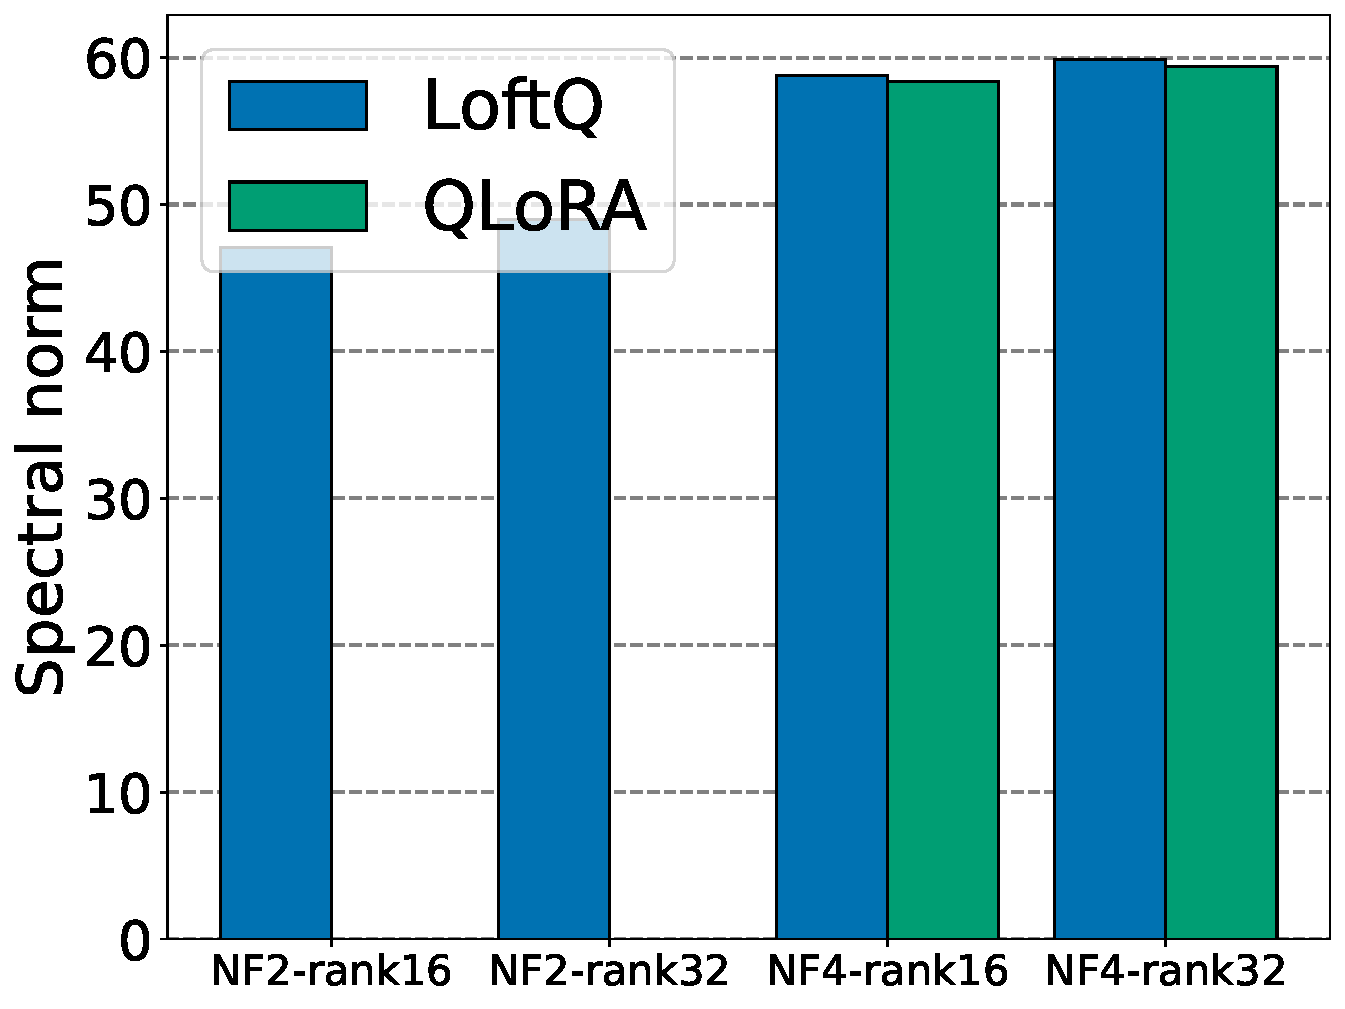
\includegraphics[width=0.48\textwidth]{figures/anli.pdf}
% \vspace{-4mm}
% \caption{ANLI}


% \vspace{-2mm}
% \caption{
% Results with {\OurAlg} of DeBERTaV3-base models trained on ANLI and evluated on all ANLI test set using NF4 and NF2 quantization. We report the median over four seeds. Results with {\it N.A.} indicate the model does not converge. The best results on each dataset are shown in bold.
% }
% \vspace{-1mm}
% \label{fig:quant_error}
% \end{figure}

% \begin{table*}[t!]
% \caption{Results with {\OurAlg} of DeBERTaV3-base models trained on ANLI and evluated on all ANLI test set using NF4 quantization. We report the median over four seeds. Results with {\it N.A.} indicate the model does not converge. The best results on each dataset are shown in bold.}
% % \vspace{-1mm}
% \label{tab:anli_experiemnts}
% \begin{center}
% \begin{tabular}{l|cccccc}
% \toprule
% {\bf Rank} & {\bf Rank16} & {\bf Rank32} \\
% \midrule
% {\bf Full FT} & \multicolumn{2}{c}{59.8} \\
% \midrule
% {\bf LoRA} & \multicolumn{2}{c}{60.2}  \\
% \midrule
% {\bf 4-bit}& \\
% % {Movement}  & \emph{N.A.} & \emph{N.A.} & \emph{N.A.} &  \emph{N.A.} &  \emph{N.A.} &  \emph{N.A.}\\
% {- QLoRA}   & 58.4  & 59.4   \\
% {- \OurAlg} & {\bf 58.8 } & {\bf  59.9}\\
% \midrule
% {\bf 2-bit} & \multicolumn{2}{c}{} \\ 

% {- QLoRA} & \emph{N.A.} & \emph{N.A.} \\
% {- \OurAlg} & {\bf 47.1}  & {\bf 49.0}  
% \\
% \bottomrule
% \end{tabular}
% \end{center}

% \end{table*}

% \begin{table*}[t!]
% \caption{Results with {\OurAlg} of DeBERTaV3-base models trained on ANLI and evluated on all ANLI test set using NF4 quantization. We report the median over four seeds. The best results on each dataset are shown in bold.}
% % \vspace{-1mm}
% \label{tab:anli_squad_experiemnts}
% \begin{center}
% \begin{tabular}{l|cc|ccc}

% \toprule
% \multicolumn{3}{c}{ANLI} & \multicolumn{3}{c}{SQuAD}\\
% \toprule
% {\bf Rank} & {\bf Rank16} & {\bf Rank32}  & {\bf Rank16} & {\bf Rank32} \\
% \midrule
% {\bf Full FT} & \multicolumn{2}{c}{59.8}  & \multicolumn{2}{c}{87.7/93.5}\\
% \midrule
% {\bf 4-bit}& \multicolumn{2}{c}{}  & \multicolumn{2}{c}{SQuAD} \\
% % {Movement}  & \emph{N.A.} & \emph{N.A.} & \emph{N.A.} &  \emph{N.A.} &  \emph{N.A.} &  \emph{N.A.}\\
% {- QLoRA}   & 58.4  & 59.4   & \multicolumn{2}{c}{SQuAD} \\
% {- \OurAlg} & {\bf 58.8 } & {\bf  59.9} & \multicolumn{2}{c}{SQuAD}\\
% \midrule
% {\bf 2-bit} & \multicolumn{2}{c}{} & \multicolumn{2}{c}{SQuAD} \\ 

% {- QLoRA} & \emph{N.A.} & \emph{N.A.}  & \multicolumn{2}{c}{SQuAD}\\
% {- \OurAlg} & {\bf 47.1}  & {\bf 49.0}   & \multicolumn{2}{c}{SQuAD}
% \\
% \bottomrule
% \end{tabular}
% \end{center}

% \end{table*}



\subsection{Encoder-Decoder Model: BART}
\textbf{Models and Datasets.} We quantize BART-large model \citep{lewis-etal-2020-bart}  with {\OurAlg}, then finetune and evaluate the model on two commonly used summarization datasets: XSum \citep{Narayan2018xsum} and CNN/DailyMail\citep{hermann2015teaching}.

\noindent \textbf{Implementation Details.} We apply {\OurAlg} to weight matrices in MHA and FFN of both encoder and decoder layers. We report ROUGE 1/2/L scores, which are the metrics for summarization tasks \citep{lin-2004-rouge}. We conduct quantization experiments in both 2-bit and 4-bit scenarios. We experiment with both NormalFloat and the uniform quantization in both 2-bit and 4-bit scenarios. In each precision, we choose rank equal to 8 and 16 for a fair comparison with the full precision LoRA baseline \citep{zhang2023adaptive}. Please see Appendix \ref{sec:app_summarization} for detailed configurations.

\noindent \textbf{Main Results.} Table \ref{tab:bart_summerization_bit4} summarizes our 4-bit quantization experiment results on the XSum and CNN/DailyMail test sets. Our method consistently outperforms QLoRA at both ranks on both datasets. It even surpasses full precision LoRA at both ranks on Xsum. We will discuss this unexpected results in Section \ref{sec:discussion}. The 2-bit quantization results are shown in Table \ref{tab:bart_summerization_bit2}. Our observation is consistent with the NLU experiments, that {\OurAlg} demonstrates the convergence to reasonable results, while QLoRA does not converge. This indicates our method is robuster by narrowing the initialization gap. 

\begin{table}[htb!]
% \vspace{-2mm}
\caption{Results with 4-bit {\OurAlg} of BART-large on XSum and CNN/DailyMail. We report ROUGE-1/2/L, the higher the better. \textit{Lead-3} means choosing the first 3 sentences as the summary. {\it N.A.} indicates the model does not converge. \textit{Full FT} refers to the full fine-tuning where all parameters are tuned. We report the median over five seeds.}
\label{tab:bart_summerization_bit4}
\vspace{-4mm}
\begin{center}
\begin{small}
\begin{tabular}{c|c|c|cc}
\toprule
{\bf Quantization} & {\bf Rank} & {\bf Method} & {\bf XSum} & {\bf CNN/DailyMail} \\ 
\midrule 
\multirow{4}*{Full Precision} & \multirow{2}*{-} & {Lead-3} & {16.30/1.60/11.95} & {40.42/17.62/36.67}  \\
~  & ~ & {Full FT} & {45.14/22.27/37.25} & {44.16/21.28/40.90} \\ \cmidrule{2-5}
~ & {8} & {LoRA} & {43.40/20.20/35.20} & {44.72/21.58/41.84} \\
~ & {16} & {LoRA} & {43.95/20.72/35.68} & {45.03/21.84/42.15} \\
\midrule
\multirow{4}*{NF4} & \multirow{2}*{8} & {QLoRA} & {42.91/19.72/34.82} & {43.10/20.22/40.06} \\
~ & ~ & {\OurAlg} & {\bf 44.08/20.72/35.89} & {\bf 43.81/20.95/40.84} \\ \cmidrule{2-5}
~ & \multirow{2}*{16} & {QLoRA} & {43.29/20.05/35.15} & {43.42/20.62/40.44} \\
~ & ~ & {\OurAlg} & {\bf 44.51/21.14/36.18} & {\bf 43.96/21.06/40.96} \\
\midrule
\multirow{4}*{Uniform} & \multirow{2}*{8} & {QLoRA} & {41.84/18.71/33.74} & {N.A.} \\
~ & ~ & {\OurAlg} & {\bf 43.86/20.51/35.69} & {\bf 43.73/20.91/40.77} \\ \cmidrule{2-5}
~ & \multirow{2}*{16} & {QLoRA} & {42.45/19.36/34.38} & {43.00/20.19/40.02} \\
~ & ~ & {\OurAlg} & {\bf 44.29/20.90/36.00} & {\bf 43.87/20.99/40.92} \\
\bottomrule
\end{tabular}
\end{small}
\end{center}
\end{table}

\begin{table}[htb!]
% \vspace{-2mm}
\caption{Results with 2-bit {\OurAlg} of BART-large on XSum and CNN/DailyMail using {\bf NF2 quantization}. {\it N.A.} indicates the model does not converge. We report ROUGE-1/2/L, the higher the better. We report the median over five seeds.}
\label{tab:bart_summerization_bit2}
\vspace{-4mm}
\begin{center}
\begin{small}
\begin{tabular}{c|c|cc}
\toprule
{\bf Rank} & {\bf Method} & {\bf XSum} & {\bf CNN/DailyMail} \\ 
\midrule 
\multirow{2}*{8} & {QLoRA} & {N.A.} &  {N.A.} \\
~  & {\OurAlg} &  {39.63/16.65/31.62} &  {42.24/19.44/29.04} \\ 
\midrule
\multirow{2}*{16} & {QLoRA} &  {N.A.} &  {N.A.} \\
~  & {\OurAlg} &  {40.81/17.85/32.80} &  {42.52/19.81/39.51} \\

\bottomrule
\end{tabular}
\end{small}
\end{center}
\end{table}


\subsection{Decoder-only Model: LLAMA-2}
\textbf{Models and Datasets.} We quantize LLAMA-2-7b and LLAMA-2-13b \citep{touvron2023llama} with {\OurAlg}. We then fine-tune and evaluate the models on two NLG datasets: GSM8K \citep{cobbe2021training} and WikiText-2 \citep{merity2016pointer}. Please see Appendix~\ref{sec:app_NLG} for more details about the datasets.

\noindent \textbf{Implementation Details.} Similarly, we apply {\OurAlg} to weight matrices in MHA and FFN of all layers. In WikiText-2 evaluation, we report perplexity. In GSM8K evaluation, we extract numerical answers in the generated solutions and then calculate the accuracy using those numerical answers. We conduct experiments with both NF2 and NF4. Please see Appendix~\ref{sec:app_NLG} for detailed configurations.

\noindent \textbf{Main Results.} 
Table \ref{tab:llama} presents a summary of our experiments on LLAMA-2-7b and LLAMA-2-13b using 2-bit, 4-bit, and mixed-precision NormalFloat quantization methods on WikiText-2 and GSM8K datasets. In WikiText-2, our method consistently outperforms QLoRA across all quantization precision settings on both models. 
% For instance, when using 4-bit precision, {\OurAlg} achieves a perplexity of 5.24 for LLAMA-2-7b, surpassing even the performance of 16-bit precision LoRA. 
When dealing with the challenging 2-bit precision, where QLoRA fails to converge, {\OurAlg} manages to achieve a perplexity of 7.85. In GSM8K, our method achieves better or on par performance compared to QLoRA across different model sizes and quantization precision levels. For example, our method achieves 20.9\% accuracy using 2-bit precision, where QLoRA doesn't converge. 

We find {\OurAlg} outperforms full precision LoRA in GSM8K with LLAMA-2-13b. One possible explanation is that the lack of regularization causes overfitting on full precision LoRA fine-tuning. Therefore, we conduct full precision LoRA with weight decay on GSM8K. From Table \ref{tab:llama}, regularization helps LLAMA-2-13b full precision LoRA fine-tuning, but fails in LLAMA-2-7b. This indicates LLAMA-2-13b is prone to overfitting and quantization has implicit regularization to overcome such overfitting.

To provide a customized trade-off between the performance and precision, we also explore mixed-precision quantization where matrices in the first 4 layers are quantized using 4 bits, and the rest matrices remain 2 bits. We witness a remarkable 5.9\% accuracy boost on the GSM8K dataset using LLAMA-2-7b and a 12.7\% boost using LLAMA-2-13b. This result underscores the potential of {\OurAlg} for complex mixed-precision quantization scenarios.
% \begin{table}[htb!]
% % \vspace{-2mm}
% \caption{Results of {\OurAlg} using 4-bit and 2-bit normal float quantization of LLAMA-2 series on WikiText-2. We report perplexity (the lower the better). The rank of low-rank adapters is 64. Results with {\it N.A.} indicate the model does not converge.}
% \label{tab:llama_wikitext}
% \vspace{-4mm}
% \begin{center}
% \begin{small}
% \begin{tabular}{cccc}
% \toprule
% {\bf Method} & {\bf Bit} & {\bf LLAMA-2-7b} & {\bf LLAMA-2-13b} \\ 
% \midrule 
% {LoRA} & {16} & {5.31} &  {5.12} \\
% \midrule
% {QLoRA}   & {4} & {7.41} & {5.22} \\
% {\OurAlg} & {4} & {\bf 5.24} & {\bf 5.16} \\ 
% \midrule 
% {QLoRA}   & {2} & {N.A.} & {N.A.} \\
% {\OurAlg} & {2} & {\bf 7.85} & {\bf 7.69} \\ 
% \bottomrule
% \end{tabular}
% \end{small}
% \end{center}
% \end{table}

\begin{table}[htb!]
\vspace{-2mm}
\caption{Results of {\OurAlg} using NormalFloat for LLAMA-2 series on WikiText-2 and GSM8K. 3/2.5/2.25-bit indicates mixed-precision quantization: 4-bit precision for the first 16/8/4 layers and 2-bit precision for the rest of layers. We report the perplexity (the smaller the better) for WikiText-2 and accuracy for GSM8K. The rank of low-rank adapters is 64. {\it N.A.} indicates the model does not converge. We report the median over five random seeds.}

\vspace{-4mm}
\label{tab:llama}
\begin{center}
\begin{small}
\begin{tabular}{cc|cccc}
\toprule
\multirow{2}*{\bf Method} & \multirow{2}*{\bf Bit} & \multicolumn{2}{c}{\bf LLAMA-2-7b} & \multicolumn{2}{c}{\bf LLAMA-2-13b} \\ 
 ~ & ~ & {\bf WikiText-2}$\downarrow$ & {\bf GSM8K}$\uparrow$ & {\bf WikiText-2}$\downarrow$  & {\bf GSM8K}$\uparrow$\\
\midrule 
{LoRA} & {16} & {5.08} & {36.9} & {5.12} & {43.1} \\
{LoRA+Reg} & {16} & {--} & {34.4} & {--} & {45.3} \\
\midrule
{QLoRA}   & {4} & {5.70} & {\bf 35.1} & {5.22} & {39.9} \\
{\OurAlg} & {4} & {\bf 5.24} & {35.0} & {\bf 5.16} & {\bf 45.0} \\ 
\midrule
{QLoRA}   & {3} & {5.73} & {32.1} & {5.22} & {40.7} \\
{\OurAlg} & {3} & {\bf 5.63} & {\bf 32.9} & {\bf 5.13} & {\bf 44.4} \\ 
\midrule 
{QLoRA}   & {2.5} & {N.A.} & {N.A.} & {19.39} & {N.A.} \\
{\OurAlg} & {2.5} & {5.78} & {\bf 31.1} & {5.22} & {\bf 41.1} \\ 
\midrule 
{QLoRA}   & {2.25} & {N.A.} & {N.A.} & {N.A.} & {N.A.} \\
{\OurAlg} & {2.25} & {\bf 6.13} & {\bf 26.5} & {\bf 5.45} & {\bf 38.1} \\ 
\midrule 

{QLoRA}   & {2} & {N.A} & {N.A.} & {N.A.} & {N.A.} \\
{\OurAlg} & {2} & {\bf 7.85} & {\bf 20.9} & {\bf 7.69} & {\bf 25.4} \\ 
\bottomrule
\end{tabular}
\end{small}
\end{center}
\end{table}

% \vspace{-4mm}
% \label{tab:llama_gsmk8k}
% \begin{center}
% \begin{small}
% \begin{tabular}{cccc}
% \toprule
% {\bf Method} & {\bf Bit} & {\bf LLAMA-2-7b} & {\bf LLAMA-2-13b} \\ 
% \midrule 
% {LoRA} & {16} & {36.9} &  {36.5} \\
% \midrule
% {QLoRA}   & {4} & {\bf 35.1} & {39.9} \\
% {\OurAlg} & {4} & {35.0} & {\bf 45.0} \\ 
% \midrule 
% {QLoRA}   & {2.25} & {N.A.} & {N.A.} \\
% {\OurAlg} & {2.25} & {\bf 26.5} & {\bf 38.1} \\ 
% \midrule 
% {QLoRA}   & {2} & {N.A.} & {N.A.} \\
% {\OurAlg} & {2} & {\bf 20.9} & {\bf 25.4} \\ 
% \bottomrule
% \end{tabular}
% \end{small}
% \end{center}
% \end{table}


\subsection{Analysis}
\textbf{Effectiveness of Alternating Optimization.}
We conduct experiments with different alternating step $T$ to verify the effectiveness of the alternating optimization and to find the best value $T$ as a hyperparameter for different models. 
Across all tasks and models, we observed that alternating optimization yields substantial improvements even with a minimal alternating step. This suggests that it rapidly narrows the discrepancy between quantized weights and pre-trained weights, making our method easy to apply. For example, our method achieves 88.0\% accuracy on MNLI-m dataset using only 5 alternating steps and 21.14 Rouge-2 score using only 1 step. Interestingly, we noticed that increasing the alternating step beyond a certain point tends to result in diminishing returns. We suspect this phenomenon occurs because, as the gap becomes smaller, it becomes more challenging for alternating optimization to consistently minimize the gap at each step. This challenge emerges because of the inherent errors introduced by the quantization method. Nevertheless, results from Figure \ref{fig:num_iter} indicate our method is not sensitive to the alternating step $T$ and is able to consistently enhance downstream fine-tuning performance.
% We remark  Figure \ref{fig:num_iter} shows that our method consistently outperforms the baseline across all tested iteration settings on different models. 
% We observed that different models achieve their best results with varying numbers of iterations, yet the performance remains stable across different numbers of iterations.
% This indicates our method is not sensitive to the number of iterations, while consistently enhancing downstream fine-tuning performance.

\begin{figure}[htb]
\centering
\begin{subfigure}{0.32\columnwidth}
    \centering
    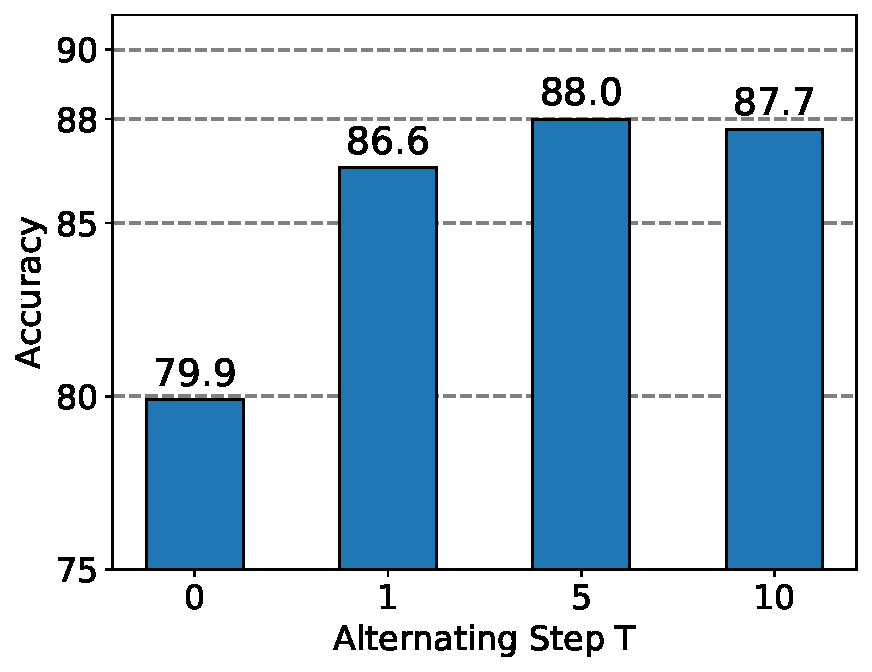
\includegraphics[width=1.0\textwidth]{figures/deberta2-mnli-uniform-bit2.pdf}
    \vspace{-5mm}
    \caption{MNLI}
\end{subfigure}
\begin{subfigure}{0.32\columnwidth}
    \centering
    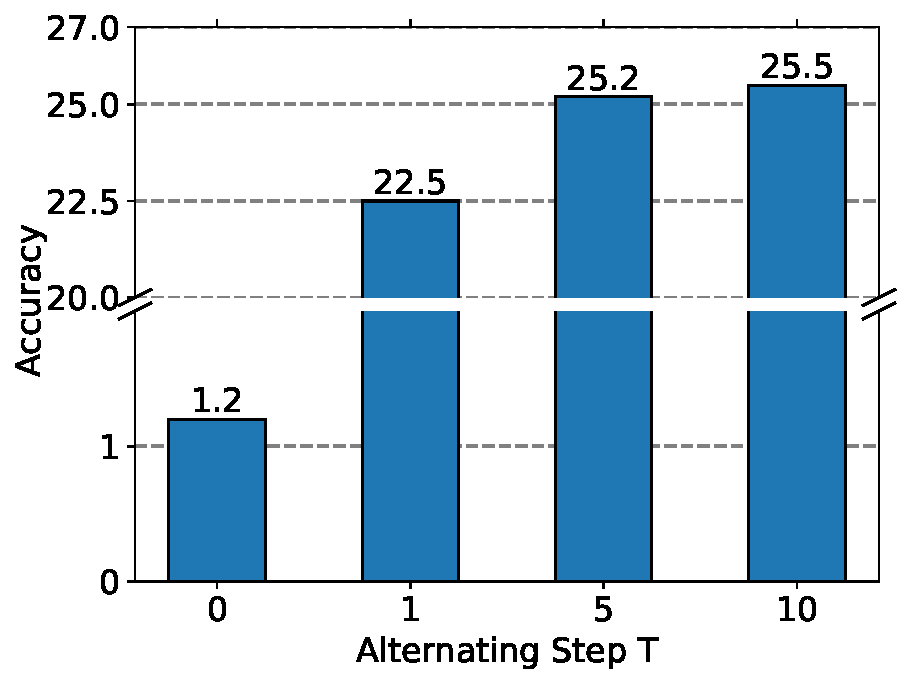
\includegraphics[width=1.0\textwidth]{figures/llama2-nf2-gsm8k.pdf}
    \vspace{-5mm}
    \caption{GSM8k}
\end{subfigure}
\begin{subfigure}{0.32\columnwidth}
    \centering
    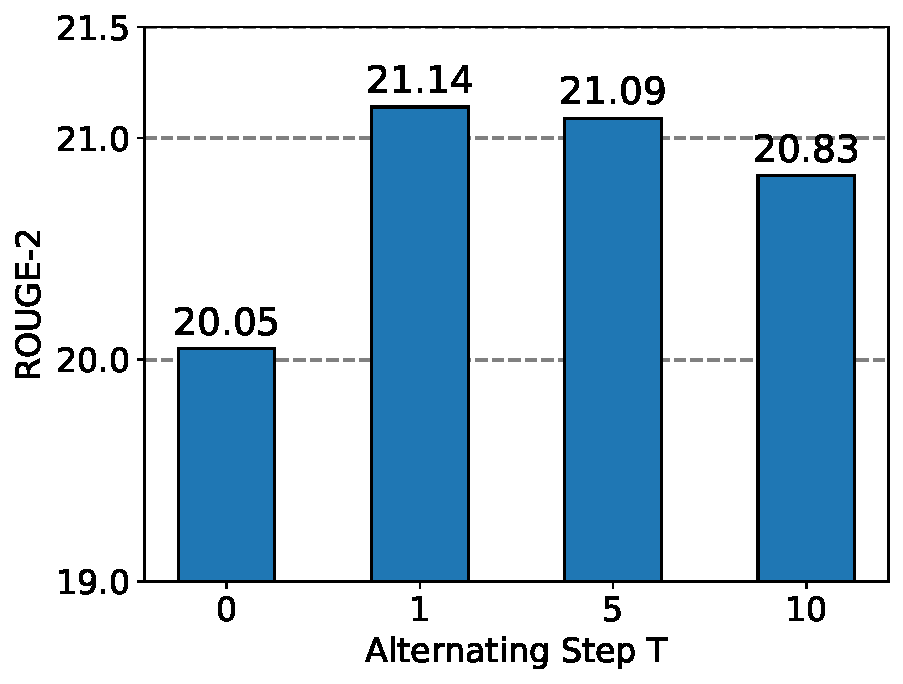
\includegraphics[width=1.0\textwidth]{figures/bart2-xsum-nf-bit4.pdf}
    \vspace{-5mm}
    \caption{XSum}
\end{subfigure}
\vspace{-2mm}
\caption{
Comparison of different alternating step $T$ used in {\OurAlg}. $T=0$ indicates we use QLoRA method that initializes low-rank adapters by \eqref{eq:lora_init}. $T = 1, 5, 10 $ indicates we use different $T$ for {\OurAlg} described in Algorithm \ref{alg:alter}. {\bf Left}: Uniform 2-bit DeBERTaV3-base. {\bf Middle}: NF4 2-bit LLAMA-2-13b. {\bf Right}: NF4 BART-large.
}
\label{fig:num_iter}
\end{figure}

